\documentclass[11pt]{article}

\usepackage[margin=1in]{geometry}
\usepackage{setspace}
\usepackage{graphicx}
\usepackage{booktabs}
\usepackage{tabularx}
\usepackage{array}
\usepackage{float}
\usepackage{amsmath}
\usepackage{hyperref}
\usepackage{caption}
\usepackage{longtable}

\setstretch{1.5}
\hypersetup{
    colorlinks=true,
    linkcolor=blue,
    citecolor=blue,
    urlcolor=blue
}

\title{\textbf{ShiftGuard: Event Aware Distribution Shift Detection Attribution and Human in the Loop Adaptation for Non Stationary Forex Markets}}
\author{
Anusha Ravi Kumar \\ \texttt{ravikumar.anu@northeastern.edu}
\and
Sohan Mahesh \\ \texttt{mahesh.so@northeastern.edu}
\and
Disha Manubhai Patel \\ \texttt{patel.dishabe@northeastern.edu}
}
\date{CS 6140 \quad Machine Learning \\ Northeastern University, Silicon Valley}

\begin{document}
\maketitle

\section{Objectives and Significance}
Financial markets are non stationary: the relationship between inputs and outcomes changes over time because of scheduled macroeconomic releases, policy decisions, geopolitical shocks, volatility dislocations, and changing trader behavior. A forecasting model that performs well in one regime can degrade quickly in another. In practice, this means that prediction accuracy by itself is not enough. A deployed model also needs to recognize when the data distribution has shifted, explain what changed, and adapt its downstream behavior.

Our motivation is also slightly different from the usual trading framing. Many systems try to predict every market move and then trade as often as possible. In this project we focus instead on understanding where we are positioned in the market, how strong the current momentum and regime context are, and whether the situation justifies a risk managed trade at all. The goal is not to take every possible trade. The goal is to take fewer but more confident trades than an always on strategy that participates in every period.

The goal of ShiftGuard is to build an end to end machine learning system for handling this problem in forex markets. Rather than framing the project as ``predict the next return and stop there,'' we treat return prediction as only one component of a larger pipeline. ShiftGuard trains a monitored model, detects scheduled and unexpected shifts, explains them using SHAP based feature attribution, supports review through a dashboard, and adapts trade posture after approved shifts. The project focuses on three instruments with distinct behavior profiles: EURUSD, GBPJPY, and XAUUSD.

This project is significant for two reasons. First, it addresses a real systems problem in applied ML: how to keep a model useful when the world around it changes. Second, it combines ideas that are often studied separately, concept drift detection, model explanation, human in the loop review, and adaptive policy selection, into one coherent workflow. Prior work has studied concept drift and adaptation broadly \cite{gama2014survey, lu2019review}, explanation techniques such as SHAP \cite{lundberg2017shap}, and human in the loop workflows \cite{monarch2021hitl, amershi2014power}, but our angle is to connect these ideas in an event aware financial pipeline where shift type and dominant cause influence trade selection and model adaptation.

\section{Background}
Concept drift refers to a change in the statistical relationship between inputs and targets over time. In financial markets, drift is especially common because market participants react to monetary policy, inflation releases, employment data, risk off events, and cross asset sentiment shocks. A single static model can therefore become stale even when its architecture is strong. Surveys by Gama et al. \cite{gama2014survey} and Lu et al. \cite{lu2019review} describe this problem and review strategies such as explicit drift detection, weighting recent data more heavily, and retraining models after regime changes.

ShiftGuard uses three forms of drift monitoring. The first is \textit{scheduled shift detection}, which targets known high impact economic releases. The second is \textit{unexpected shift detection}, which tries to catch non calendar disruptions such as flash moves or geopolitical events. The third is \textit{performance drift detection}, which monitors the model's prediction errors directly. This combination is motivated by the fact that a market can change both because of known external events and because of changes that are not visible in a calendar.

Interpretability is another major part of the project. When a shift is detected, the next question is not only \textit{did something change?} but also \textit{what changed?} TreeSHAP provides a practical way to explain tree based models by decomposing predictions into feature contributions \cite{lundberg2017shap}. In ShiftGuard, these feature level contributions are aggregated into broader groups, technical, volatility, macro, and sentiment, to explain which type of information dominated a shift. This matters because different causes may call for different responses.

The project is also motivated by human in the loop ML. In many high stakes or noisy settings, automatic detection alone is not enough; human review can improve trust, prevent false positives, and guide corrective action. Monarch \cite{monarch2021hitl} and Amershi et al. \cite{amershi2014power} emphasize that human input is most valuable when the system presents interpretable evidence and keeps review lightweight. ShiftGuard follows this philosophy with a dashboard that makes the pipeline visible through four main analytic views and a separate review panel, while still allowing a person to override a decision when needed.

What makes our work particularly interesting is the way these pieces are connected. ShiftGuard is not just a predictor, not just a drift detector, and not just a dashboard. It is a pipeline where a monitored XGBoost regressor provides predictions for drift monitoring, detected shifts are explained using SHAP, reviewed shifts can guide adaptation decisions, and the same shift context also informs a regime filtered trading policy. The project therefore studies adaptation as a system level behavior rather than as a single algorithmic trick.

\section{Methods}
\subsection{Data and Task Definition}
The project uses three instruments: EURUSD, GBPJPY, and XAUUSD. The canonical price series are stored as 4 hour OHLCV bars in \texttt{data/raw/price/}. The repository also includes utilities for downloading full historical hourly prices from Dukascopy and shorter range hourly prices from Yahoo Finance \cite{dukascopy, yfinance}. In the current setup, the price history spans approximately January 2015 through April 2026 before preprocessing.

In addition to price data, ShiftGuard uses curated macroeconomic calendar data, daily interest rate and yield information, sentiment and cross asset signals, and manually assembled event context files. The raw folders include per currency economic calendars, daily macro files, daily VIX/DXY/SP500/oil sentiment features, daily news volume, and gold specific sentiment factors for XAUUSD. These are merged into pair level feature matrices in \texttt{data/processed/}.

Before final modeling, we explored the pair level data to understand volatility scale event density and missing value behavior. This exploration showed that XAUUSD had larger and less stable return magnitudes than EURUSD, while GBPJPY and XAUUSD displayed stronger sensitivity to sentiment and event context. These observations motivated both the multi group feature design and the decision to evaluate each pair separately instead of forcing one shared response profile across all instruments.

The modeling task is next bar return prediction on 4 hour bars. For each pair, the target variables are:
\begin{itemize}
    \item \texttt{target\_return}: next 4H log return
    \item \texttt{target\_direction}: binary direction of the next return
\end{itemize}
The regression target is canonical for the project because it provides a continuous error stream for drift monitoring and more interpretable recovery analysis after shifts.

\subsection{Data Processing and Feature Engineering}
We build processed feature matrices using four main feature groups:
\begin{itemize}
    \item \textbf{Technical:} moving averages and momentum indicators along with MACD ADX RSI stochastic indicators Williams \%R CCI ROC band features ATR Keltner channels and bar return structure
    \item \textbf{Volatility:} Garman Klass volatility Parkinson volatility rolling standard deviations volatility of volatility volatility ratios and drawdown features
    \item \textbf{Macro:} rate differentials yield spreads yield curve event surprise event count days to next high impact event and binary flags for rate decisions NFP and CPI
    \item \textbf{Sentiment / cross asset:} VIX DXY S\&P 500 return oil return rolling correlations news volume spikes and gold specific factors for XAUUSD
\end{itemize}

Each processed pair is built from chronologically ordered 4 hour bars. Macro and sentiment sources are merged by date and forward filled across intraday bars. The pipeline drops the first 60 bars as warm up because rolling indicators are undefined at the start of the series, and it drops the last row because the next bar target is unavailable there. The resulting dataset sizes are reported in Table \ref{tab:model_summary}. The final processed feature counts are 70 features for EURUSD, 70 for GBPJPY, and 76 for XAUUSD.

\subsection{Pipeline Overview}
Figure \ref{fig:pipeline_overview} summarizes the end to end workflow.

\begin{figure}[H]
\centering
\fbox{
\parbox{0.92\linewidth}{
\centering
\textbf{Raw Data} $\rightarrow$ \textbf{Feature Engineering} $\rightarrow$ \textbf{Monitored Model (XGBoost)} $\rightarrow$ \textbf{Shift Detection} $\rightarrow$ \textbf{SHAP Attribution} $\rightarrow$ \textbf{Dashboard / HITL Review} $\rightarrow$ \textbf{Selective Retraining + Adaptive Trading} $\rightarrow$ \textbf{Evaluation}
}
}
\caption{High level ShiftGuard workflow.}
\label{fig:pipeline_overview}
\end{figure}

The repository supports full pipeline regeneration through:
\begin{center}
\texttt{python src/run\_all\_phases.py --clean}
\end{center}
This command rebuilds datasets, reruns the monitored model, runs detection and attribution, materializes default review decisions, executes selective retraining, refreshes trading comparisons, and regenerates summary figures. The reported results in this project were generated through this end to end wrapper rather than through a manually stepped interactive run. In particular, \texttt{src/run\_all\_phases.py} calls the core pipeline \texttt{src/run\_pipeline.py} with \texttt{--auto-confirm-decisions} enabled so that detected shifts are materialized into approved decisions and then passed into selective retraining without manual intervention. This benchmark choice was made to keep the reported regeneration path fully reproducible and internally consistent.

\subsection{Monitored Model and Baselines}
The canonical monitored model is an \texttt{XGBRegressor} trained on next bar return. The train/validation/test split is chronological with a 70/15/15 ratio. Hyperparameters are tuned on the training segment using a 5 fold \texttt{TimeSeriesSplit} and mean absolute error (MAE) as the objective. The search grid includes:
\begin{itemize}
    \item \texttt{learning\_rate} $\in \{0.01, 0.05, 0.1\}$
    \item \texttt{max\_depth} $\in \{3,5,7\}$
    \item \texttt{n\_estimators} $\in \{300,500\}$
    \item \texttt{reg\_alpha} $\in \{0, 0.1, 1.0\}$
    \item \texttt{reg\_lambda} $\in \{1.0, 5.0\}$
\end{itemize}

We chose XGBoost as the canonical model because it offers a useful balance of predictive strength interpretability and runtime. It is fast enough to tune repeatedly across pairs, compatible with exact TreeSHAP explanations, and simple to retrain after shifts. We also experimented with more complex supporting baselines locally, including stacked and sequence based models, but those did not offer the same combination of explanation quality reproducibility and practical rerun speed for the final submission path.

The tuned configurations also reflect pair specific differences in complexity. EURUSD selected a deeper model with learning rate 0.05 and depth 5, GBPJPY selected a shallower depth 3 model with learning rate 0.01, and XAUUSD selected a deeper depth 5 model with stronger regularization. This is important because it shows that hyperparameter tuning was not treated as a formality; the project uses pair specific model settings rather than one copied configuration for all instruments.

We compare ShiftGuard against two main baselines:
\begin{itemize}
    \item \textbf{Technical baseline:} a rule based RSI/MACD trading benchmark
    \item \textbf{ML Direction baseline:} an always on XGBoost directional strategy without explicit shift aware control
\end{itemize}
These baselines test whether handcrafted signals or plain predictive learning are sufficient without the larger shift aware system.

\subsection{Shift Detection}
Shift detection has three components.

\paragraph{Scheduled shifts.}
For known high impact macro releases, we align each event timestamp to the nearest available 4 hour feature bar and compare the pre event and post event windows. The implementation uses 60 bars before and 60 bars after each event. It runs a Kolmogorov Smirnov (KS) test per feature and a Maximum Mean Discrepancy (MMD) score on the full feature vector. High impact events are retained only if they exceed statistical thresholds, which prevents the detector from flagging nearly every calendar event. In simplified form,
\[
\mathrm{MMD}^2(X,Y) =
\frac{1}{m^2} \sum_{i,j} k(x_i, x_j)
+ \frac{1}{n^2} \sum_{i,j} k(y_i, y_j)
- \frac{2}{mn} \sum_{i,j} k(x_i, y_j),
\]
where $k(\cdot, \cdot)$ is an RBF kernel and $X, Y$ are pre and post event samples.

\paragraph{Unexpected shifts.}
Unexpected shifts are detected on non event days using ADWIN \cite{bifet2007adwin}, which maintains an adaptive window over feature streams and signals when the mean changes enough to justify a cut. In our implementation, the detector uses $\delta=0.002$ and ignores days already associated with high impact scheduled events.

\paragraph{Performance drift.}
Performance drift is measured directly from the monitored model's prediction stream using the Drift Detection Method (DDM) \cite{gama2004ddm}. Directional prediction errors are converted into a binary error stream. A warning is raised when
\[
p_t + s_t \ge p_{\min} + 2 s_{\min},
\]
and drift is raised when
\[
p_t + s_t \ge p_{\min} + 3 s_{\min},
\]
after a minimum number of observations. This allows the pipeline to catch not only feature space changes, but also true degradation in predictive behavior.

\subsection{Shift Attribution and Dashboard / HITL Review}
After shift detection, ShiftGuard runs TreeSHAP on post shift samples around each detected event \cite{lundberg2017shap}. Feature level SHAP values are aggregated into four interpretable groups: technical, volatility, macro, and sentiment. The dominant group acts as an explanation of what type of information most likely drove the shift.

These explanations are displayed in a Streamlit dashboard. The dashboard includes four main visualization sections titled Overview, P\&L Simulator, Price and Regimes, and Shift Detection, plus a separate Review Shifts panel that allows manual inspection of flagged events. The review workflow supports:
\begin{itemize}
    \item confirm
    \item reject
    \item override review notes
    \item retraining queue inspection
\end{itemize}
For the reported experiments, detected shifts were automatically materialized into approved decisions and then passed into retraining because the submission facing wrapper ran the core pipeline with \texttt{--auto-confirm-decisions} enabled. The standard pipeline still supports human review and manual override through the dashboard, but those interactive overrides were not used in the benchmark configuration reported here. At this stage, human reclassification is mainly used for visual inspection and audit. Feeding reclassified labels directly back into retraining remains future work because the system would first need a reliable way to validate reviewer corrections and map those corrected labels to the right retraining action such as full retrain or weighted retrain.

\subsection{Selective Retraining and Adaptive Trading}
Reviewed shifts feed into selective retraining. We compare five policies:
\begin{enumerate}
    \item No retrain
    \item Full retrain
    \item Window retrain (30 day local window)
    \item Weighted retrain (recent data emphasized)
    \item Adaptive retrain (policy selected from shift type and dominant SHAP group)
\end{enumerate}

Retraining is evaluated over a 180-bar post-shift horizon using rolling MAE and recovery bars, where recovery means the model returns to its pre-shift error level.

The same shift context also drives an adaptive trading policy. Technical dominant shifts favor a technical follow through posture. Scheduled shifts dominated by macro or sentiment features favor broader event aware participation. Unexpected or volatility led shifts trigger more defensive behavior. This is an important design choice: the project tests whether the \emph{reason} for a shift should influence the system's response.

\subsection{Evaluation Strategy}
Evaluation is multi layered rather than relying on a single score:
\begin{itemize}
    \item \textbf{Prediction metrics:} MAE RMSE directional accuracy classification accuracy precision recall and F1
    \item \textbf{Detection metrics:} counts of scheduled unexpected and performance shifts
    \item \textbf{Attribution metrics:} dominant feature group patterns across shifts
    \item \textbf{Retraining metrics:} average post shift MAE recovery bars and percent recovered
    \item \textbf{Trading metrics:} win rate profit factor cumulative return market participation profit from a fixed capital simulation and ending balance
    \item \textbf{Portfolio metrics:} combined profit and ending balance when capital is allocated across all three instruments
    \item \textbf{Statistical comparison:} paired $t$ tests between the technical baseline and ShiftGuard on overlapping trades
\end{itemize}

\section{Experiments, Results, and Analysis}
We report five main experiments in this section. Experiment 1 compares ShiftGuard against trading baselines. Experiment 2 interprets the same trade logs through fixed capital profits and a combined portfolio view. Experiment 3 evaluates retraining after approved shifts. Experiment 4 adds a stricter walk forward robustness evaluation for the canonical monitored model. Experiment 5 is an ablation study that isolates the value of major pipeline components. We also present monitored model and detection results first because they provide the evidence chain for the downstream decisions. Unless noted otherwise, the results below come from the reproducible end to end regeneration path in \texttt{src/run\_all\_phases.py}, which calls \texttt{src/run\_pipeline.py} with \texttt{--auto-confirm-decisions} enabled and does not use manual dashboard overrides.

\subsection{Monitored Model Performance}
Table \ref{tab:model_summary} summarizes the monitored XGBoost regressor on the held out test split for all three instruments.

\begin{table}[H]
\centering
\caption{Canonical monitored-model summary on the chronological test split.}
\label{tab:model_summary}
\resizebox{\textwidth}{!}{
\begin{tabular}{lcccccc}
\toprule
Pair & Features & Train Rows & Val Rows & Test Rows & Test MAE & Directional Accuracy \\
\midrule
EURUSD & 70 & 12{,}670 & 2{,}715 & 2{,}715 & 0.001141 & 59.52\% \\
GBPJPY & 70 & 12{,}669 & 2{,}715 & 2{,}715 & 0.001621 & 52.63\% \\
XAUUSD & 76 & 12{,}572 & 2{,}694 & 2{,}694 & 0.003483 & 51.37\% \\
\bottomrule
\end{tabular}
}
\end{table}

EURUSD is the strongest of the three on raw predictive metrics, while XAUUSD is the hardest forecasting problem. This variation is useful because it tests whether the rest of the ShiftGuard system adds value even when prediction quality differs by pair.

\subsection{Shift Detection and Attribution Results}
Table \ref{tab:detection_summary} reports the shift counts produced by the detection engine and the dominant feature group explanations from SHAP attribution.

\begin{table}[H]
\centering
\caption{Detected shifts and dominant attribution patterns.}
\label{tab:detection_summary}
\resizebox{\textwidth}{!}{
\begin{tabular}{lccccc}
\toprule
Pair & Scheduled & Unexpected & Performance Drift & Total Shifts & Dominant Attribution Pattern \\
\midrule
EURUSD & 26 & 5 & 0 & 31 & Technical on 31/31 shifts \\
GBPJPY & 7 & 19 & 1 & 27 & Sentiment on 27/27 shifts \\
XAUUSD & 27 & 23 & 0 & 50 & Sentiment on 34/50, Technical on 16/50 \\
\bottomrule
\end{tabular}
}
\end{table}

These results are informative in their own right. EURUSD appears to be driven mainly by technical structure shifts in the current run, while GBPJPY and XAUUSD are more sensitive to sentiment and event context. This supports the intuition that different pairs experience different types of non stationarity, so a single adaptation rule is unlikely to be optimal.

\subsection{Experiment 1: Baseline vs. ShiftGuard Trading Comparison}
Our first main experiment compares three downstream trading policies:
\begin{enumerate}
    \item Technical baseline (RSI/MACD)
    \item ML Direction baseline (always on XGBoost)
    \item ShiftGuard (regime filtered and shift aware policy)
\end{enumerate}

Figure \ref{fig:winrate_comparison} visualizes market participation across pairs, and Table \ref{tab:trading_summary} reports the exact numbers.

\begin{figure}[H]
\centering
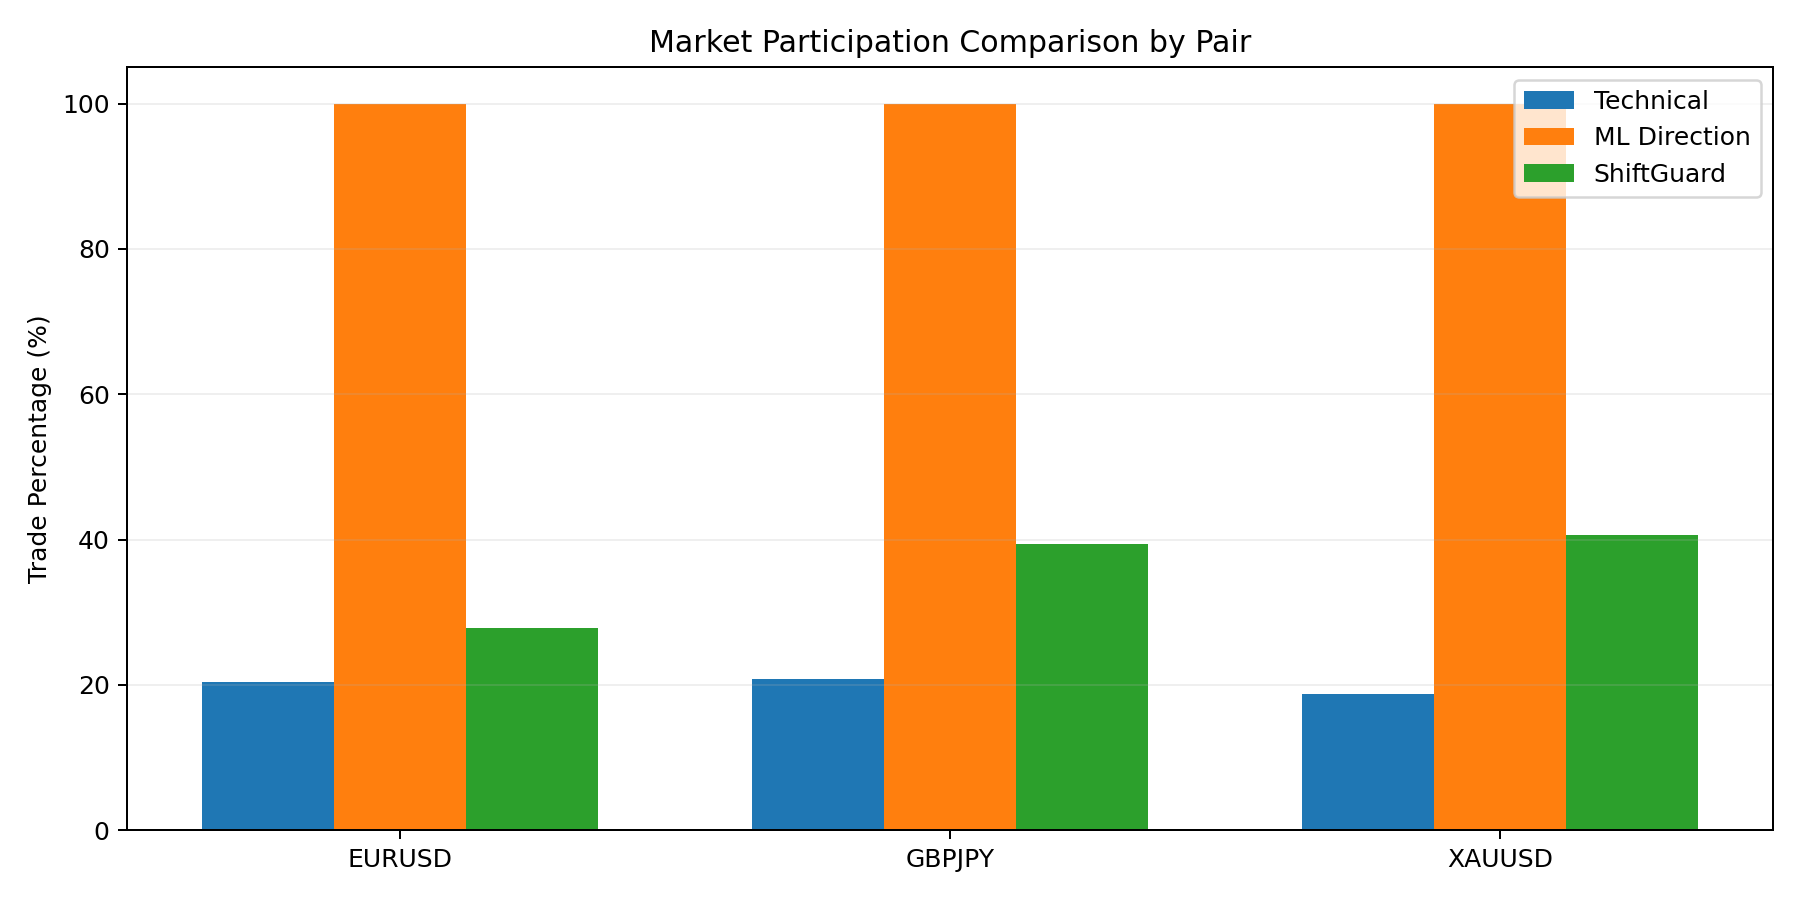
\includegraphics[width=0.88\textwidth]{results/figures/winrate_comparison.png}
\caption{Risk managed comparison across pairs using trade percentage or market participation for the technical baseline, ML Direction baseline, and ShiftGuard.}
\label{fig:winrate_comparison}
\end{figure}

\begin{table}[H]
\centering
\caption{Trading comparison between baselines and ShiftGuard. Cumulative return is the raw summed return from the simulator, and trade \% is market participation.}
\label{tab:trading_summary}
\resizebox{\textwidth}{!}{
\begin{tabular}{llcccc}
\toprule
Pair & Strategy & Win Rate & Profit Factor & Cumulative Return & Trade \% \\
\midrule
EURUSD & Technical (RSI/MACD) & 50.86\% & 1.02 & 0.051953 & 20.4 \\
EURUSD & ML Direction (XGBoost) & 56.68\% & 1.80 & 6.039058 & 100.0 \\
EURUSD & ShiftGuard & 58.45\% & 2.14 & 2.539135 & 28.1 \\
\midrule
GBPJPY & Technical (RSI/MACD) & 50.92\% & 1.13 & 0.360118 & 20.8 \\
GBPJPY & ML Direction (XGBoost) & 52.15\% & 1.10 & 1.436116 & 100.0 \\
GBPJPY & ShiftGuard & 59.01\% & 1.98 & 4.444332 & 39.5 \\
\midrule
XAUUSD & Technical (RSI/MACD) & 50.11\% & 0.95 & -0.179178 & 18.7 \\
XAUUSD & ML Direction (XGBoost) & 49.95\% & 1.02 & 0.489408 & 100.0 \\
XAUUSD & ShiftGuard & 58.01\% & 1.89 & 5.850500 & 40.6 \\
\bottomrule
\end{tabular}
}
\end{table}

This experiment shows that ShiftGuard is the strongest overall downstream system on GBPJPY and XAUUSD. It produces the highest win rate and the highest profit factor on both pairs, while also substantially outperforming the technical baseline. The market participation figure adds the key risk managed interpretation: the ML Direction baseline trades all the time, while ShiftGuard participates in a much smaller share of periods and still delivers stronger trade quality. On EURUSD, ShiftGuard still achieves the best win rate and profit factor, but the always on ML baseline has the highest cumulative return because it trades continuously. This is an important interpretation point: ShiftGuard is more selective by design, so it emphasizes signal quality and regime filtering rather than raw trade frequency.

\begin{figure}[H]
\centering
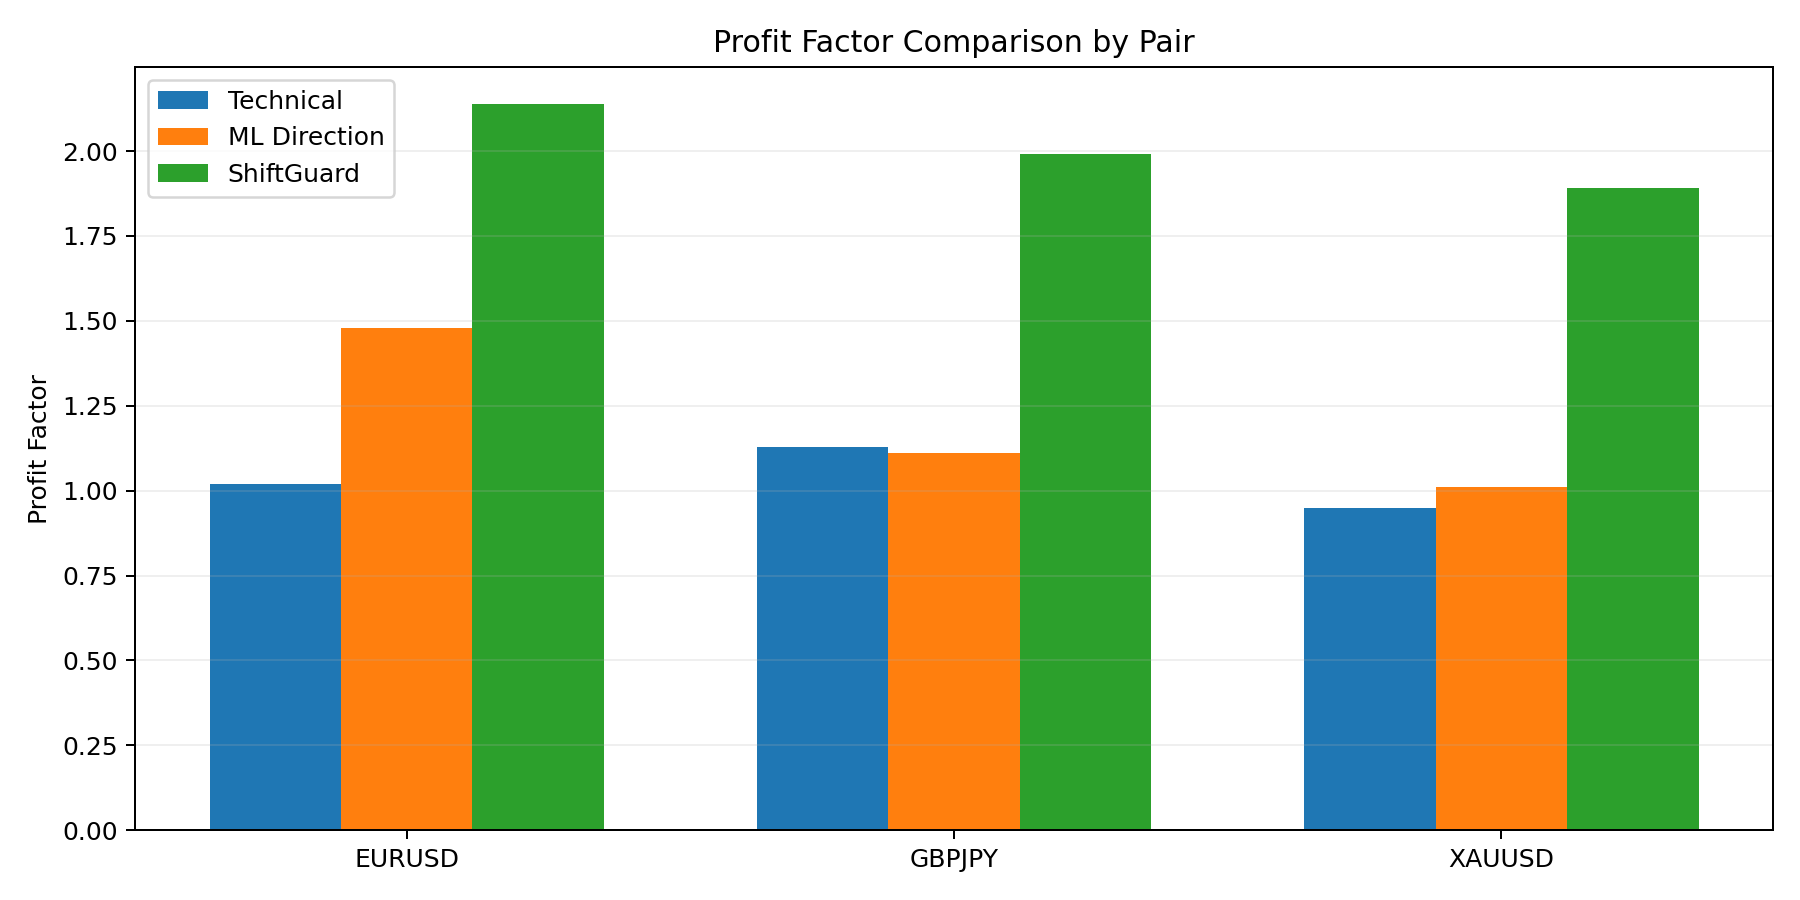
\includegraphics[width=0.88\textwidth]{results/figures/profit_factor_comparison.png}
\caption{Profit factor comparison across pairs for the technical baseline, ML Direction baseline, and ShiftGuard.}
\label{fig:profit_factor_comparison}
\end{figure}

We also tested whether the improvement over the technical baseline is statistically meaningful. Table \ref{tab:stats} shows that the paired comparison is significant for all three pairs.

\begin{table}[H]
\centering
\caption{Paired statistical comparison between the technical baseline and ShiftGuard on overlapping trades.}
\label{tab:stats}
\begin{tabular}{lccc}
\toprule
Pair & Technical Win Rate & ShiftGuard Win Rate & $p$-value \\
\midrule
EURUSD & 60.18\% & 62.58\% & 0.003182 \\
GBPJPY & 58.13\% & 60.83\% & 0.000045 \\
XAUUSD & 55.27\% & 59.56\% & $< 10^{-6}$ \\
\bottomrule
\end{tabular}
\end{table}

\subsection{Experiment 2: Fixed Capital Profit and Portfolio Analysis}
To make the trading comparison more concrete, we converted the same trade logs into a fixed capital P\&L interpretation using \$10{,}000 starting capital per pair, 1:20 leverage, transaction cost deductions, a 30\% tax on profits, and a 1\% stop loss cap in the current simulator for EURUSD, GBPJPY, and XAUUSD. Because trading quality is not fully captured by win rate alone, we treat profit and ending balance as core results alongside win rate and profit factor. Table \ref{tab:investment_balances} reports the resulting ending balances across horizons.

\begin{table}[H]
\centering
\caption{Ending balance from a \$10{,}000 starting investment per pair. Assumptions: 1:20 leverage fixed trading cost approximation 30\% tax on profits and a 1\% stop loss cap in the simulator.}
\label{tab:investment_balances}
\resizebox{\textwidth}{!}{
\begin{tabular}{llccc}
\toprule
Pair & Horizon & Technical End Balance & ML Direction End Balance & ShiftGuard End Balance \\
\midrule
EURUSD & 1M & \$10{,}619 & \$12{,}820 & \$12{,}622 \\
EURUSD & 3M & \$8{,}709 & \$15{,}094 & \$16{,}484 \\
EURUSD & 6M & \$6{,}705 & \$18{,}642 & \$16{,}729 \\
EURUSD & 1Y & \$5{,}863 & \$49{,}363 & \$31{,}294 \\
EURUSD & 2Y & \$363 & \$75{,}188 & \$53{,}699 \\
EURUSD & 5Y & \$0 & \$247{,}728 & \$127{,}441 \\
\midrule
GBPJPY & 1M & \$7{,}682 & \$4{,}047 & \$12{,}772 \\
GBPJPY & 3M & \$3{,}934 & \$0 & \$15{,}505 \\
GBPJPY & 6M & \$0 & \$0 & \$17{,}231 \\
GBPJPY & 1Y & \$0 & \$0 & \$26{,}874 \\
GBPJPY & 2Y & \$0 & \$0 & \$73{,}235 \\
GBPJPY & 5Y & \$0 & \$0 & \$165{,}605 \\
\midrule
XAUUSD & 1M & \$10{,}447 & \$32{,}657 & \$29{,}531 \\
XAUUSD & 3M & \$1{,}574 & \$32{,}331 & \$71{,}526 \\
XAUUSD & 6M & \$0 & \$4{,}477 & \$91{,}068 \\
XAUUSD & 1Y & \$0 & \$0 & \$137{,}912 \\
XAUUSD & 2Y & \$0 & \$0 & \$165{,}632 \\
XAUUSD & 5Y & \$0 & \$0 & \$283{,}817 \\
\bottomrule
\end{tabular}
}
\end{table}

In profit terms, the same table shows why ShiftGuard is important as a trading system rather than only as a classifier or regressor wrapper. By 3 months, ShiftGuard grows \$10{,}000 to \$16{,}484 on EURUSD, \$15{,}505 on GBPJPY, and \$71{,}526 on XAUUSD. By 6 months, those balances become \$16{,}729, \$17{,}231, and \$91{,}068. By 1 year, they become \$31{,}294, \$26{,}874, and \$137{,}912. This fixed capital view reinforces the earlier conclusions. ShiftGuard is the most robust strategy on GBPJPY and XAUUSD, where the two baselines frequently collapse to zero under realistic leverage and cost assumptions while ShiftGuard remains profitable. On EURUSD, the always on ML baseline reaches a larger ending balance, but ShiftGuard remains materially profitable with much lower market participation and stronger trade quality metrics.

A balance of \$0 in Table \ref{tab:investment_balances} does not mean every trade failed. It means that under the leveraged simulator, repeated losses after transaction costs eventually exhausted the initial \$10{,}000 and the balance was clipped at zero rather than allowed to become negative. This is why some baselines still show positive win rates in earlier tables but still reach \$0 over longer horizons.

Because a realistic trader may allocate capital across multiple instruments, we also evaluated a combined portfolio with \$10{,}000 assigned to each pair for a total starting capital of \$30{,}000. Table \ref{tab:portfolio_balances} reports the resulting portfolio balances.

\begin{table}[H]
\centering
\caption{Combined portfolio ending balance with \$10{,}000 allocated to each pair for a total starting capital of \$30{,}000.}
\label{tab:portfolio_balances}
\begin{tabular}{lccc}
\toprule
Horizon & Technical Portfolio & ML Direction Portfolio & ShiftGuard Portfolio \\
\midrule
1M & \$29{,}205 & \$51{,}309 & \$54{,}926 \\
3M & \$14{,}217 & \$50{,}425 & \$103{,}515 \\
6M & \$6{,}705 & \$26{,}822 & \$125{,}028 \\
1Y & \$5{,}863 & \$55{,}363 & \$196{,}080 \\
2Y & \$363 & \$81{,}188 & \$292{,}566 \\
5Y & \$0 & \$253{,}728 & \$576{,}863 \\
\bottomrule
\end{tabular}
\end{table}

The portfolio view strengthens the same conclusion. With \$10{,}000 allocated to each pair, the total ShiftGuard portfolio value reaches \$103{,}515 after 3 months, \$125{,}028 after 6 months, and \$196{,}080 after 1 year. This is important because it shows that the advantage of selective positioning is not limited to one pair. It carries through even when the strategy is evaluated as a diversified portfolio.

Figure \ref{fig:equity_curves} provides a more intuitive view of how these strategies accumulate returns over time.

\begin{figure}[H]
\centering
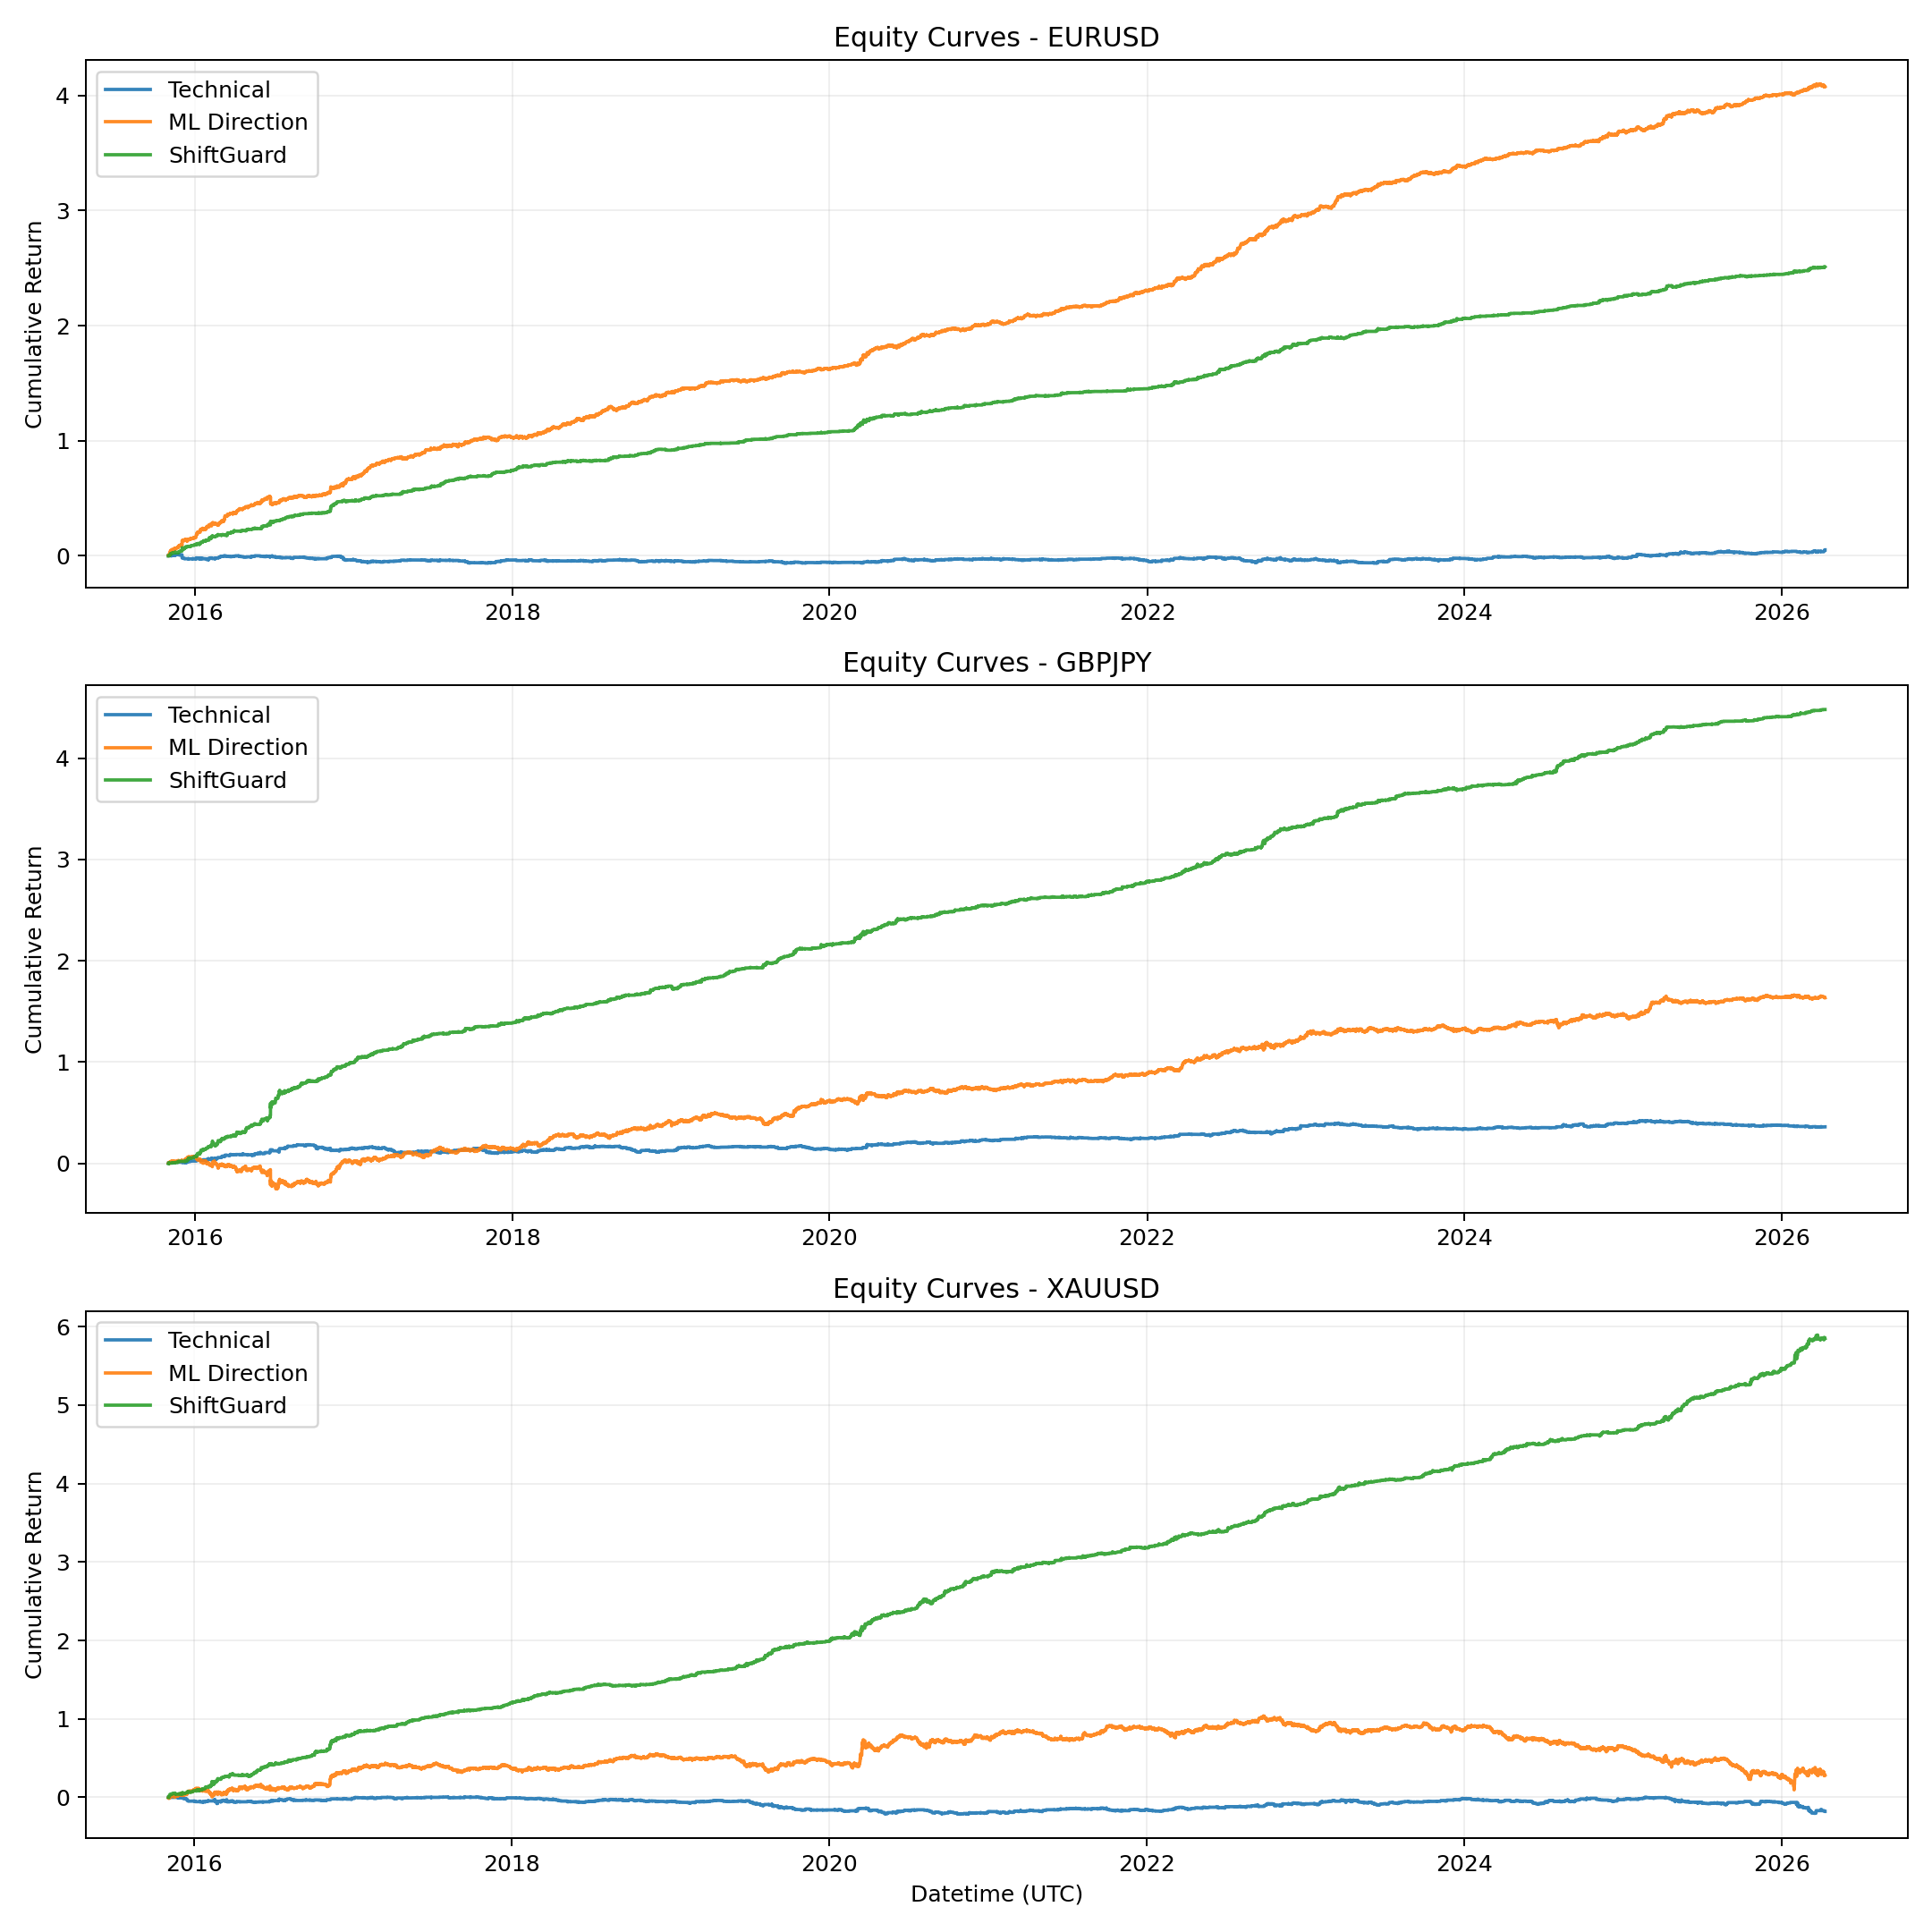
\includegraphics[width=0.94\textwidth]{results/figures/equity_curves.png}
\caption{Equity curves for the technical baseline, ML Direction baseline, and ShiftGuard on each pair.}
\label{fig:equity_curves}
\end{figure}

\subsection{Experiment 3: Selective Retraining After Approved Shifts}
Our third main experiment tests whether retraining after approved shifts improves recovery relative to doing nothing. We compare five policies: no retrain, full retrain, 30 day window retrain, weighted retrain, and adaptive retrain. Table \ref{tab:retraining_summary} summarizes the pair level results.

\begin{table}[H]
\centering
\caption{Selective retraining summary. Lower MAE is better and lower recovery bars are better.}
\label{tab:retraining_summary}
\resizebox{\textwidth}{!}{
\begin{tabular}{lcccc}
\toprule
Pair & No Retrain MAE / Recovered \% & Best Strategy & Best MAE & Recovery Bars / Recovered \% \\
\midrule
EURUSD & 0.001180 / 85.7\% & Full Retrain & 0.001173 & 43.0 / 85.7\% \\
GBPJPY & 0.001652 / 85.7\% & Full or Adaptive & 0.001643 & 70.7 / 85.7\% \\
XAUUSD & 0.004181 / 76.9\% & Weighted & 0.004148 & 54.9 / 84.6\% \\
\bottomrule
\end{tabular}
}
\end{table}

The retraining results are more nuanced than the trading results. Retraining helps, but not uniformly. On EURUSD and GBPJPY, full retraining gives only a small MAE improvement over doing nothing. On XAUUSD, weighted retraining performs best and also improves the share of recovered shifts. We therefore treat retraining as a promising but still developing part of the project rather than the strongest finished claim.

\subsection{Experiment 4: Walk-Forward Robustness Evaluation}
The first three experiments use a static chronological holdout split, which is appropriate for a clean reproducible benchmark but still trains the monitored model only once before the test period. To test whether the same monitored model remains stable under a stricter temporal protocol, we ran an additional expanding-window walk forward experiment on the canonical \texttt{XGBRegressor}. Starting at the 2021 evaluation boundary, the model was refit before each 180 bar block using only data available up to that point, and the resulting rolling predictions were concatenated into one walk forward evaluation stream. Table \ref{tab:walkforward_summary} compares the current single-fit holdout benchmark against this walk forward setup.

\begin{table}[H]
\centering
\caption{Walk-forward robustness comparison for the canonical monitored model. Lower MAE is better and higher directional accuracy is better.}
\label{tab:walkforward_summary}
\resizebox{\textwidth}{!}{
\begin{tabular}{lccccc}
\toprule
Pair & Holdout MAE & Walk-Forward MAE & Holdout Directional Accuracy & Walk-Forward Directional Accuracy & Refit Windows \\
\midrule
EURUSD & 0.001141 & 0.001122 & 59.34\% & 60.87\% & 48 \\
GBPJPY & 0.001621 & 0.001636 & 52.45\% & 53.10\% & 48 \\
XAUUSD & 0.003483 & 0.002632 & 51.34\% & 55.84\% & 47 \\
\bottomrule
\end{tabular}
}
\end{table}

\begin{figure}[H]
\centering
\includegraphics[width=0.95\textwidth]{results/figures/walkforward_metric_comparison.png}
\caption{Static holdout versus walk-forward comparison on MAE and directional accuracy for each pair.}
\label{fig:walkforward_metric_comparison}
\end{figure}

Figure \ref{fig:walkforward_metric_comparison} makes the main robustness result easier to read than the table alone. The walk-forward protocol improves directional accuracy on all three pairs, while the MAE bars show that XAUUSD benefits the most from repeated refits and GBPJPY changes only marginally. This is the most useful walk-forward visualization for the main report because it summarizes the headline comparison in one view.

The walk forward results strengthen the project in two ways. First, they show that the canonical monitored model does not collapse when evaluated under repeated refits with strictly past-only data. Directional accuracy improves on all three pairs, and MAE improves on two of the three pairs. Second, the gains are clearly pair dependent rather than universal. EURUSD improves modestly, GBPJPY is roughly neutral on MAE while still gaining a small accuracy lift, and XAUUSD benefits the most by a wide margin. This is a useful robustness result because it supports the claim that non stationarity matters most on the harder, more unstable instrument. It also gives us a more defensible answer when asked whether the reported holdout results are overly optimistic: under a stricter walk forward setup, the monitored model remains competitive and in one case becomes materially better.

\begin{figure}[H]
\centering
\includegraphics[width=0.92\textwidth]{results/figures/walkforward_rolling_mae.png}
\caption{Rolling 90-bar MAE across the evaluation window for the static holdout and walk-forward protocols.}
\label{fig:walkforward_rolling_mae}
\end{figure}

Figure \ref{fig:walkforward_rolling_mae} adds temporal detail by showing where the two evaluation protocols diverge over time. The curves largely track each other on EURUSD and GBPJPY, which supports the claim that walk-forward evaluation is stable rather than erratic, while XAUUSD shows larger error swings and the clearest benefit from repeated adaptation. This figure is more diagnostic than summary-oriented, so it works best as a supporting figure when space allows.

\subsection{Experiment 5: Ablation Study}
The report includes two ablation style studies that isolate the value of individual parts of the system.

\paragraph{System level ablation.}
Table \ref{tab:trading_summary} can be read as a staged component ablation:
\begin{itemize}
    \item \textbf{Technical baseline:} no learned model and no shift detection attribution or adaptive response
    \item \textbf{ML Direction baseline:} learned model only with no explicit shift aware filtering or adaptation
    \item \textbf{ShiftGuard:} learned model plus shift detection plus attribution plus review layer plus adaptive response
\end{itemize}
Under this view, the gap between the ML Direction baseline and ShiftGuard measures the value of adding shift aware control on top of a predictive model. The results show that these added components improve win rate profit factor and fixed capital profit consistently across all three pairs, with the clearest gains on GBPJPY and XAUUSD.

\paragraph{Adaptation policy ablation.}
Table \ref{tab:retraining_summary} acts as an ablation over adaptation choices after a shift. Here, the monitored model and detection pipeline are fixed, while the retraining response is varied across no retrain full retrain local window retrain weighted retrain and adaptive retrain. This isolates which part of the response policy actually matters after a detected shift. The results show that a response policy is useful, but also that the best policy is pair dependent: full retraining is strongest on EURUSD and GBPJPY, while weighted retraining is strongest on XAUUSD.

\paragraph{Ablation takeaway.}
Together, these ablations support two claims. First, the full ShiftGuard pipeline adds value beyond a plain predictive model. Second, adaptation itself is not one dimensional: once a shift is detected, the choice of response still matters, and different markets benefit from different retraining strategies. The walk forward experiment adds a third perspective: the monitored model itself is reasonably robust under stricter time-aware evaluation, but repeated updating is most beneficial on the pair with the strongest observed non stationarity.

\subsection{Interpretation, Limitation, and Surprising Result}
One important observation is that end to end trading quality depends on more than raw predictive accuracy. XAUUSD had the weakest held out forecasting accuracy of the three pairs, yet ShiftGuard produced its strongest downstream trading gains there. This suggests that the project is gaining value from selective positioning and regime awareness rather than from raw prediction alone.

Another useful observation is that adaptive retraining looks promising but not yet conclusive. In the current results it matches or improves upon simpler retraining choices on some pairs, but it is not yet dominant everywhere. We therefore view adaptive learning as a meaningful direction supported by the current evidence, while still leaving room for a more principled policy learning step.

The main limitations are therefore about refinement rather than contradiction. First, the trading comparison is still simulator based, so it should be treated as a controlled evaluation of relative strategy quality rather than as proof of live deployment readiness. Second, even though the new walk forward experiment is more realistic than the static holdout, it still uses fixed feature engineering and fixed model classes rather than a fully online live system. Third, earlier classifier based formulations created a circular definition issue during hyperparameter tuning because the regime labels and the classifier objective were too tightly coupled. That made interpretation less stable and was one reason we centered the final pipeline on a regressor with a separate detection and adaptation layer. Fourth, if human overrides are to be used directly as training signals in the future, the system will need a better way to validate reviewer consistency and map corrected shift types to retraining choices.

\section{Conclusions and Future Work}
ShiftGuard set out to build an ML system that detects distribution shifts in non stationary forex markets, explains them, and adapts to them through review, trading posture changes, and model update choices. Overall, the project met these goals.

There are five main takeaways. First, \textbf{shift aware filtering improves downstream trading quality}, especially on GBPJPY and XAUUSD, where ShiftGuard clearly outperformed both baselines. Second, \textbf{profit and ending balance are essential evaluation outcomes} for this project because they capture the practical effect of selective trade entry more directly than accuracy alone. At the portfolio level, with \$10{,}000 allocated to each pair, the total ShiftGuard portfolio value reaches \$103{,}515 after 3 months, \$125{,}028 after 6 months, and \$196{,}080 after 1 year. Third, \textbf{prediction accuracy by itself does not determine system success}; the full pipeline matters more than the monitored model in isolation. Fourth, \textbf{the monitored model remains competitive under stricter walk forward evaluation}, with directional accuracy improving on all three pairs and the largest MAE gain appearing on XAUUSD. Fifth, \textbf{the strongest contribution of the project is system integration}: event aware detection SHAP attribution dashboard review and adaptive response work better together than they do as disconnected components.

What worked best was the regime filtered trading layer and the strong baseline comparison story. The retraining policy layer is better described as promising than definitive, because the gains are real but still mixed across pairs. This means the project succeeded most clearly as a shift aware decision system, while the retraining component remains an area that should be refined further before being treated as a final claim.

There are several concrete directions for future work, all of them for the Research and Innovation Showcase. The first is to replace the current rule based adaptive retraining logic with a learned policy that chooses the retraining strategy from shift type dominant feature group and recent recovery history. The second is to extend the new walk forward benchmark with dynamic transaction cost stress tests and more realistic slippage assumptions, so the trading comparison better reflects evolving market conditions. The third is to design a careful feedback loop for human overrides and reclassifications, where corrected labels are validated first and then mapped to retraining actions in a principled way instead of being fed directly back into the model without checks. The fourth is to evolve ShiftGuard into a live adaptive system. In the current pipeline, the monitored XGBoost is refit in controlled walk forward batches rather than updated continuously in production. A stronger next step would be to let the system ingest new market data continuously, monitor for drift in real time, surface live shift alerts, and update retraining or trading decisions as market conditions change. This would move ShiftGuard beyond historical analysis and toward an ongoing adaptation framework for real market non stationarity.

\section{Team Contributions and Reflection}
The project was organized into eight task phases: data acquisition and cleaning; feature engineering and dataset construction; monitored model and baseline development; shift detection; shift attribution; dashboard and human in the loop review; selective retraining and adaptive trading response; and evaluation, analysis, and final delivery.

\paragraph{Disha Manubhai Patel.}
Disha led data acquisition and cleaning, including collecting and aligning raw forex, macroeconomic calendar, macro indicator, sentiment, and event context inputs. She also worked on evaluation, including comparison setup, metric generation, and helping conduct one of the project experiments. In addition, she helped identify relevant reference papers and contributed to presentation preparation.

\paragraph{Anusha Ravi Kumar.}
Anusha led feature engineering and dataset construction, including processed dataset creation, target alignment, and train/validation/test preparation. She also led monitored model and baseline development, including the main XGBoost modeling pipeline and baseline comparison systems. In addition, she built the dashboard and human in the loop review layer, including the interface for shift inspection, confirmation, rejection, relabeling, and retraining trigger decisions. She contributed to final delivery, including integration, report polishing, and presentation preparation.

\paragraph{Sohan Mahesh.}
Sohan led the shift detection pipeline, including scheduled shift detection, unexpected shift detection, and performance drift monitoring. He also led shift attribution and analysis, including SHAP based feature group attribution and interpretation of detected shifts. He led selective retraining and adaptive trading response, including retraining policy experiments and the regime filtered trading logic. He also led the evaluation analysis of how individual pipeline components affected final performance. He contributed to final delivery, including end to end pipeline integration, experiment interpretation, and presentation support.

\paragraph{Reflection.}
The team collaborated closely on interface design between stages because the project only works when outputs from one phase become reliable inputs to the next. Two recurring challenges were keeping timestamps aligned across event, prediction, and feature data, and keeping the project reproducible as the pipeline grew from a forecasting task into a full shift aware ML system. We handled this by standardizing intermediate files under \texttt{results/}, regenerating the canonical outputs from one entry point, and repeatedly aligning implementation choices with the core project goal: detecting, explaining, and adapting to non stationarity in financial markets.

This project was not simply a repackaging of a pure forecasting model. The new contribution here is the end to end shift aware system itself: event aligned detection, explanation through grouped SHAP attribution, a reviewable HITL layer, and adaptive retraining and trading decisions connected in one reproducible pipeline.

\section{References}
\begin{thebibliography}{99}

\bibitem{gama2004ddm}
Joao Gama, Pedro Medas, Gladys Castillo, and Pedro Rodrigues.
\newblock Learning with drift detection.
\newblock In \emph{Advances in Artificial Intelligence -- SBIA 2004}, 2004.

\bibitem{gama2014survey}
Joao Gama, Indre Zliobaite, Albert Bifet, Mykola Pechenizkiy, and Abdelhamid Bouchachia.
\newblock A survey on concept drift adaptation.
\newblock \emph{ACM Computing Surveys}, 46(4), 2014.

\bibitem{lu2019review}
Jie Lu, Anjin Liu, Fan Dong, Feng Gu, Joao Gama, and Guangquan Zhang.
\newblock Learning under concept drift: A review.
\newblock \emph{IEEE Transactions on Knowledge and Data Engineering}, 31(12), 2019.

\bibitem{bifet2007adwin}
Albert Bifet and Ricard Gavalda.
\newblock Learning from time-changing data with adaptive windowing.
\newblock In \emph{Proceedings of SIAM International Conference on Data Mining}, 2007.

\bibitem{chen2016xgboost}
Tianqi Chen and Carlos Guestrin.
\newblock XGBoost: A scalable tree boosting system.
\newblock In \emph{Proceedings of the 22nd ACM SIGKDD International Conference on Knowledge Discovery and Data Mining}, 2016.

\bibitem{lundberg2017shap}
Scott Lundberg and Su-In Lee.
\newblock A unified approach to interpreting model predictions.
\newblock In \emph{Advances in Neural Information Processing Systems}, 2017.

\bibitem{monarch2021hitl}
Robert Monarch.
\newblock \emph{Human-in-the-Loop Machine Learning}.
\newblock Manning, 2021.

\bibitem{amershi2014power}
Saleema Amershi, Maya Cakmak, W. Bradley Knox, and Todd Kulesza.
\newblock Power to the people: The role of humans in interactive machine learning.
\newblock \emph{AI Magazine}, 35(4), 2014.

\bibitem{yfinance}
Yahoo Finance.
\newblock \url{https://finance.yahoo.com/}.
\newblock Accessed April 2026.

\bibitem{dukascopy}
Dukascopy Historical Data Feed.
\url{https://www.dukascopy.com/swiss/english/marketwatch/historical/}.
Accessed April 2026.

\end{thebibliography}

\end{document}
